\documentclass[11pt]{article}
\usepackage{color}
\usepackage{authblk}%allows footnote format for authors
\usepackage[letterpaper, margin=1in]{geometry} %package that allows changes in margins and header/footers
\usepackage[numbers,sort]{natbib}
\usepackage{amsmath}
\usepackage{rotating}
\usepackage{adjustbox}
\usepackage[english]{babel}
\usepackage{colortbl}
\usepackage{booktabs}
\usepackage[x11names,dvipsnames,table]{xcolor}
\bibliographystyle{ieeetr}
\newcommand{\mbh}[1]{\textcolor{orange}{ \emph{\scriptsize  #1}} } %creating command for Matt's comments
\newcommand{\lwang}[1]{\textcolor{red}{ \emph{\scriptsize  #1}} } %creating command for Li's comments
\newcommand{\gmj}[1]{\textcolor{blue}{ \emph{\scriptsize  #1}} } %creating command for Garrett's comments

\title{Review: Adaptive Introgression Expanded the Genetic Base of Crops during post-Domestication Spread}

\author[1]{Authors: Garrett M. Janzen}%author information
\author[1]{Li Wang}
\author[1,*]{Matthew B. Hufford}
\affil[1]{Department of Ecology, Evolution, and Organismal Biology, Iowa State University, Ames, Iowa, USA}
\affil[*]{Correspondence: mhufford@iastate.edu (M.B. Hufford)}
\date{}

\begin{document}



\maketitle

%Short Research reviews should be in the range 3500–4000 words, with up to 40 references and 6 figures/tables.


The process of domestication is often conceptualized as geographically constrained, with crops originating from a wild progenitor within one or more defined centers followed by expansion to the modern-day extent of cultivation \cite{Harlan1992}.
However, archaeological and genetic evidence are beginning to reveal that, in many cases, domestication has been temporally protracted and geographically diffuse \cite{brown2009complex, Meyer2016, wang2017, zhou2017, Fuller2014}.
An important aspect of the emerging complexity of domestication is beneficial gene flow (\emph{i.e.}, adaptive introgression) from locally adapted wild relatives during crop expansion following initial domestication.


Adaptive introgression has three components: hybridization between two genomes, backcrossing to one of the parents, and selection on different recombinant genotypes with progressively diminished linkage drag \cite{barton2001role, Feuillet200824}.
In domesticated species, adaptive introgression would consist of crop/wild hybrids backcrossing to a crop, retention and increase in frequency of adaptive wild haplotypes in the crop, and selection against undesirable wild background.
To date, literature on crop-wild gene flow has focused on the risk of transgene introgression from domesticated crops into wild relatives (for a review, \cite{stewart2003transgene}) and on modern plant breeding efforts to introgress desired traits from wild relatives (for a review, \cite{Dempewolf2017}).
The history of natural introgression of wild alleles into domesticated crops over evolutionary timescales has received considerably less attention.
However, new tools and methods have recently been employed to detect genome-wide patterns of introgression, granting new insights into the prevalence of adaptive introgression in crop histories.
Preliminary results suggest a need to expand our conception of domestication to include a broadening of the genetic base of crops that occurred during post-domestication expansion through gene flow with newly encountered wild relatives.


In this review, we will: 1) briefly describe recently developed methods for detecting adaptive introgression and provide a summary of how they can be applied to detect crop-wild introgression, 2) present case studies suggesting wild-to-crop introgression has conferred local adaptation, 3) consider how adaptive introgression alters traditional concepts of domestication, and 4) describe future advances in both basic and applied genetics that can be made through the study of introgression in agroecosystems.


\section*{Introgression methods and their application}

\mbh{In this section, I think the overall content is good, but we need to edit to make it more accessible and more explicit about how methods are implemented to detect adaptive introgression}

The decreasing cost of genome-wide resequencing and availability of reduced-representation genotyping (\emph{e.g.}, GBS and RAD-Seq), combined with new analytical methods, has facilitated comprehensive study of introgression across a number of species (\textbf{Table 1}).
High-density marker data can be used with haplotype-based and other methods to assign specific genomic regions to a taxon of origin and identify introgression across taxa \cite{Martin2015,Price2009,Lawson2012,pease2015,rosenzweig2016,geneva2015}.
The methods reviewed here do not include those marginally estimating introgression\slash migration rate as a component of demographic history (\emph{e.g.}, Approximate Bayesian Computation (ABC) \cite{beaumont2002}, diffusion approximations for demographic inference ($\delta a\delta i$) \cite{gutenkunst2009}, isolation with migration models \cite{hey2004}, and a series of methods utilizing the sequentially Markovian coalescent (PSMC, MSMC and SMC++) \cite{li2011, schiffels2014, terhorst2017}). 
Rather, we focus on methods that explicitly identify introgressed genomic segments based on the extent of differentiation, on patterns of nucleotide/haplotype sharing, and phylogenetic relationships.
%We focus here on analytical prospects and limitations and introduce only a few representatives of each category.

First, introgressed segments are expected to show low differentiation from their source population.
The $F_{st}$ and $d_{XY}$ statistics and their derivates including $G_{min}$ \cite{geneva2015} and $RND_{min}$\cite{rosenzweig2016} gauge differentiation. 
The former two statistics are insensitive to rare migrants and therefore lack power to detect recent introgression, while the latter two overcome this limitation.
Additionally, $RND_{min}$ accounts for variable mutation rate, which is detected based on branch length to an outgroup: 

% \begin{equation}
%    G_{min} = \frac{d_{min}}{d_{XY}}
% \end{equation}
% where $d_{min}$ is the minimum sequence distance between haplotypes in species X and Y.
 
 \begin{equation}
 	RND_{min} = \frac{d_{min}}{d_{out}}
 \end{equation}
where $d_{min}$ is the minimum sequence distance between haplotypes in species X and Y and $d_{out}$ equals $(d_{XO} + d_{YO})/2$, the average sequence distance between each species and the outgroup ($O$).
 
These statistics have recently been further developed by adding differentiation between both non-admixed ($A$) and admixed populations ($B$) and a source population ($C$) \cite{racimo2016}. 
For example, the $U_{A,B,C(w,x,y)}$ statistic summarizes number of sites where an allele at frequency $y$ in the source population ($C$) has a frequency higher than $x$ in the admixed population ($B$) and lower than $w$ in the non-admixed population ($C$).
A similar statistic, $Q95_{A,B,C(w,y)}$, sets a hard cutoff at the $95^{th}$ percentile of allele frequencies in the admixed population (B) \cite{racimo2016}.
Further modifications have allowed specification of more than one source population (see details in \cite{racimo2016}).
 
Second, local ancestry deconvolution (also known as chromosome painting) assigns genomic regions to various source populations based on patterns of allele/haplotype sharing \cite{schraiber2015}. 
One form of chromosome painting utilizes hidden Markov models to evaluate ancestry across admixed genomes through comparison to reference, non-admixed individuals (\emph{e.g.}, HAPMIX \cite{Price2009}). 
Another clusters admixed populations with reference samples using a sliding-window approach (\emph{e.g.}, PCAdmix \cite{brisbin2012pcadmix} and LAMP \cite{sankararaman2008}).
And finally, introgression can be detected through chromosome painting by using a Bayesian model \cite{pritchard2000} in which deviations from Hardy-Weinberg equilibrium are minimized through creation of genetic groups (\emph{e.g.}, fineSTRUCTURE \cite{Lawson2012}). 

\gmj{Li, are you familiar with the analytical tools MIGRATE-N and BAYESASS?  Rieseberg comapres these two to STRUCTURE at some length in the discussion of this paper:
https://biology.unm.edu/Whitney/Whitney%20Reprints/Scascitelli%20et%20al%202010.pdf
Should we include these two methods, even in passing, in this portion of the paper?}

Third, the ABBA-BABA statistic (also known as the D-statistic) and its derivatives are widely applied to introgression detection.
These statistics make inferences regarding introgression based on genomic patterns of derived variants that are shared between populations or species.
Patterns of allele sharing are interpreted in a phylogenetic context and the method is best suited to detection of introgression at the genome level.
Elaborations of the D-statistic capable of localizing introgression to specific genomic regions include $\hat{f_{d}}$ \cite{Martin2015} and the five-taxon D-statistic \cite{pease2015}. 
The former is quite similar to the D-statistic but uses allele frequencies from each population/species, and the latter detects introgression based on the localized phylogenetic pattern and is capable of determining introgression directionality.

Application of these approaches across a number of plant and animal species suggests introgression can play an adaptive role. For example, introgression from ancient hominins (\emph{e.g.}, Neanderthals and Denisovans) to humans has been detected at loci controlling skin pigmentation, defense against pathogens, and toleration of high altitude (reviewed in \cite{Racimo2015}); introgression has conferred M\"{u}llerian mimicry \mbh{I would explain a bit more here...wing coloration loci, protects against predation...} across butterfly species \cite{Heliconius2012}; introgression has spread insecticide resistance across mosquito species \cite{Norris2015}, and introgression across \emph{Mimulus} (\emph{i.e.}, monkeyflower) species has resulted in adaptation to pollinator preference and contributed to speciation \cite{Stankowski2015}.






\section*{Crop adaptation through introgression}


Over the last few years, several high-profile publications based on genome-wide data have documented introgression between crops and their wild relatives outside putative domestication centers.
Recent empirical studies have revealed that introgression has occurred in many of the world's most important crops (\textbf{Table 2}).






\begin{enumerate}
\item{Maize:}






The relationship between maize (\emph{Zea mays} ssp. \emph{mays}) and the teosinte \emph{Zea mays} ssp. \emph{mexicana} (hereafter referred to as \emph{mexicana}) offers a prime case study of adaptive wild-to-crop introgression.
Maize was domesticated from \emph{Zea mays} ssp. \emph{parviglumis} (hereafter referred to as \emph{parviglumis})  approximately 9,000 years ago in the lowlands of the Balsas River Valley in Mexico \cite{matsuoka2002single}.
From this domestication center, maize spread into the highlands of the Mexican Central Plateau, where it came into sympatry with \emph{mexicana}.
Introgression from \emph{mexicana} to maize in the Central Plateau has long been reported based on both morphological \cite {wilkes1977, lauter2004, doebley1984} and molecular \cite{matsuoka2002single, vanHeerwaarden2011, doebley1987, warburton2011, fukunaga2005} data.
However, \citep{hufford2013} first localized \emph{mexicana} introgression to chromosomal regions and provided evidence that it was likely adaptive.
%The following is not fully clear.  Cut or revise.
The authors identified nine genomic regions in several maize populations which consistently showed evidence of \emph{mexicana} introgression based on chromosome painting using both HAPMIX and the linkage model of STRUCTURE (Figure \ref{fig:introgressionMaize}).
These introgressed segments showed low diversity and overlapped QTL that had previously been found to control anthocyanin content and leaf macrohairs \cite{lauter2004}, traits known to be adaptive at high elevation.
In a growth chamber experiment, the authors demonstrated that maize populations with \emph{mexicana} introgression showed greater plant height (a proxy for fitness) under highland environmental conditions than populations that lacked introgression.
Height differences were not detected under lowland conditions.
%Among the nine regions, three span the centromeres of chromosomes 5, 6, and 10, and one is located in the inversion polymorphism on chromosome 4, suggesting a significant role of genome structures restricting recombination in adaptive introgression.
%In summary, the introgressed alleles/haplotypes from \emph{mexicana} to maize conferred adaptation to highland habitats when maize migrated from Mexican lowlands.


%Even though introgression from \emph{mexicana} to Mexican highland maize has been highly supported, it is yet unknown whether and to what extent such introgression could be found in other highland maize populations which are allopatric to \emph{mexicana}. 
%A recent study \cite{Takuno2015} found little empirical or theoretical support for parallel highland adaptation in the Mexican and South American highland regions, which was explained partly by the difference in potential for adaptive introgression from wild relatives.
%Adaptive SNPs in Mexican highland population were more likely located in the introgressed regions than those in South American highland populations.
%Furthermore, the adaptive SNPs in the Mexican highland population were more likely also showing signatures of local adaptation in \emph{mexicana} and \emph {pulviglumis} populations than those South American highland population.
%For these reasons, adaptive introgression from wild relatives may play a significant role in patterning the genetic differences of maize highland populations.

Populations of \emph{mexicana} cannot be found outside of Mexico, yet maize has colonized and adapted to high elevation in a number of other regions.
%Several questions regarding \emph{mexicana} introgression yet remain.
%Has the introgression from \emph{mexicana} spread to multiple highland populations? 
%How do highland-adaptation traits differ among populations with and without introgression from \emph{mexicana}?
A recent study \cite{wang2017} employed the ABBA-BABA and $\hat{f_{d}}$ statistics to evaluate whether maize with \emph{mexicana} introgression was transferred to other highland regions or whether highland adaptation was obtained \emph{de novo} outside of Mexico.
%On chromosome 4 (Figure \ref{fig:fd}), Mexican highland (MexHigh) and Guatamalan highland (GuaHigh) exhibited strong evidence of introgression from \emph{mexicana}, and the peaks of distribution corresponded to the region identified in Hufford et al. (2013) \citep{hufford2013}.
%The signal of introgression is absent for the other three populations.
%On chromosome 5, the signals of introgression (the peak region of the distribution) are present in MexHigh, GuaHigh and Southwestern US Highland (SW\_US), but not the other two.
%More details on the other chromosomes can be found in \cite{Wang2015manuscript}.
Overall, analyses revealed that maize landraces with \emph{mexicana} introgression were transferred to nearby high elevation regions in Guatemala and the southwestern United States, but more distant high elevation regions (\emph{e.g.,} the Andes) showed no \emph{mexicana} ancestry. 
%The Andean maize, the population totally isolated from the occurrence of any teosinte species, underwent the severest historical bottleneck, as a population in the front wave of the serial founder effects. 
%The stronger genetic drift introduced by the smaller historical population size increased homozygosity but reduced the heterozygosity of the population, and it also extended the length of homozygosity.
%The high frequency of deleterious alleles caused by stronger genetic drift in the Andes population, together with the reduced efficiency of selection against deleterious sites, contributes to the observed higher mutation load in the well-isolated maize population.
%Although it is clear that the absence of introgression from wild relatives provided fewer genetic resources for highland adaptation (making the highland adaptation in the Andes unique), it is yet unknown whether or not being out of reach of wild relatives is a reason for reduced fitness in the Andes population.
%Furthermore, the question of whether convergent evolution occurs between populations with and without introgression from wild relatives is a key topic for future studies in maize.


\begin{figure}[h]
	\centering
	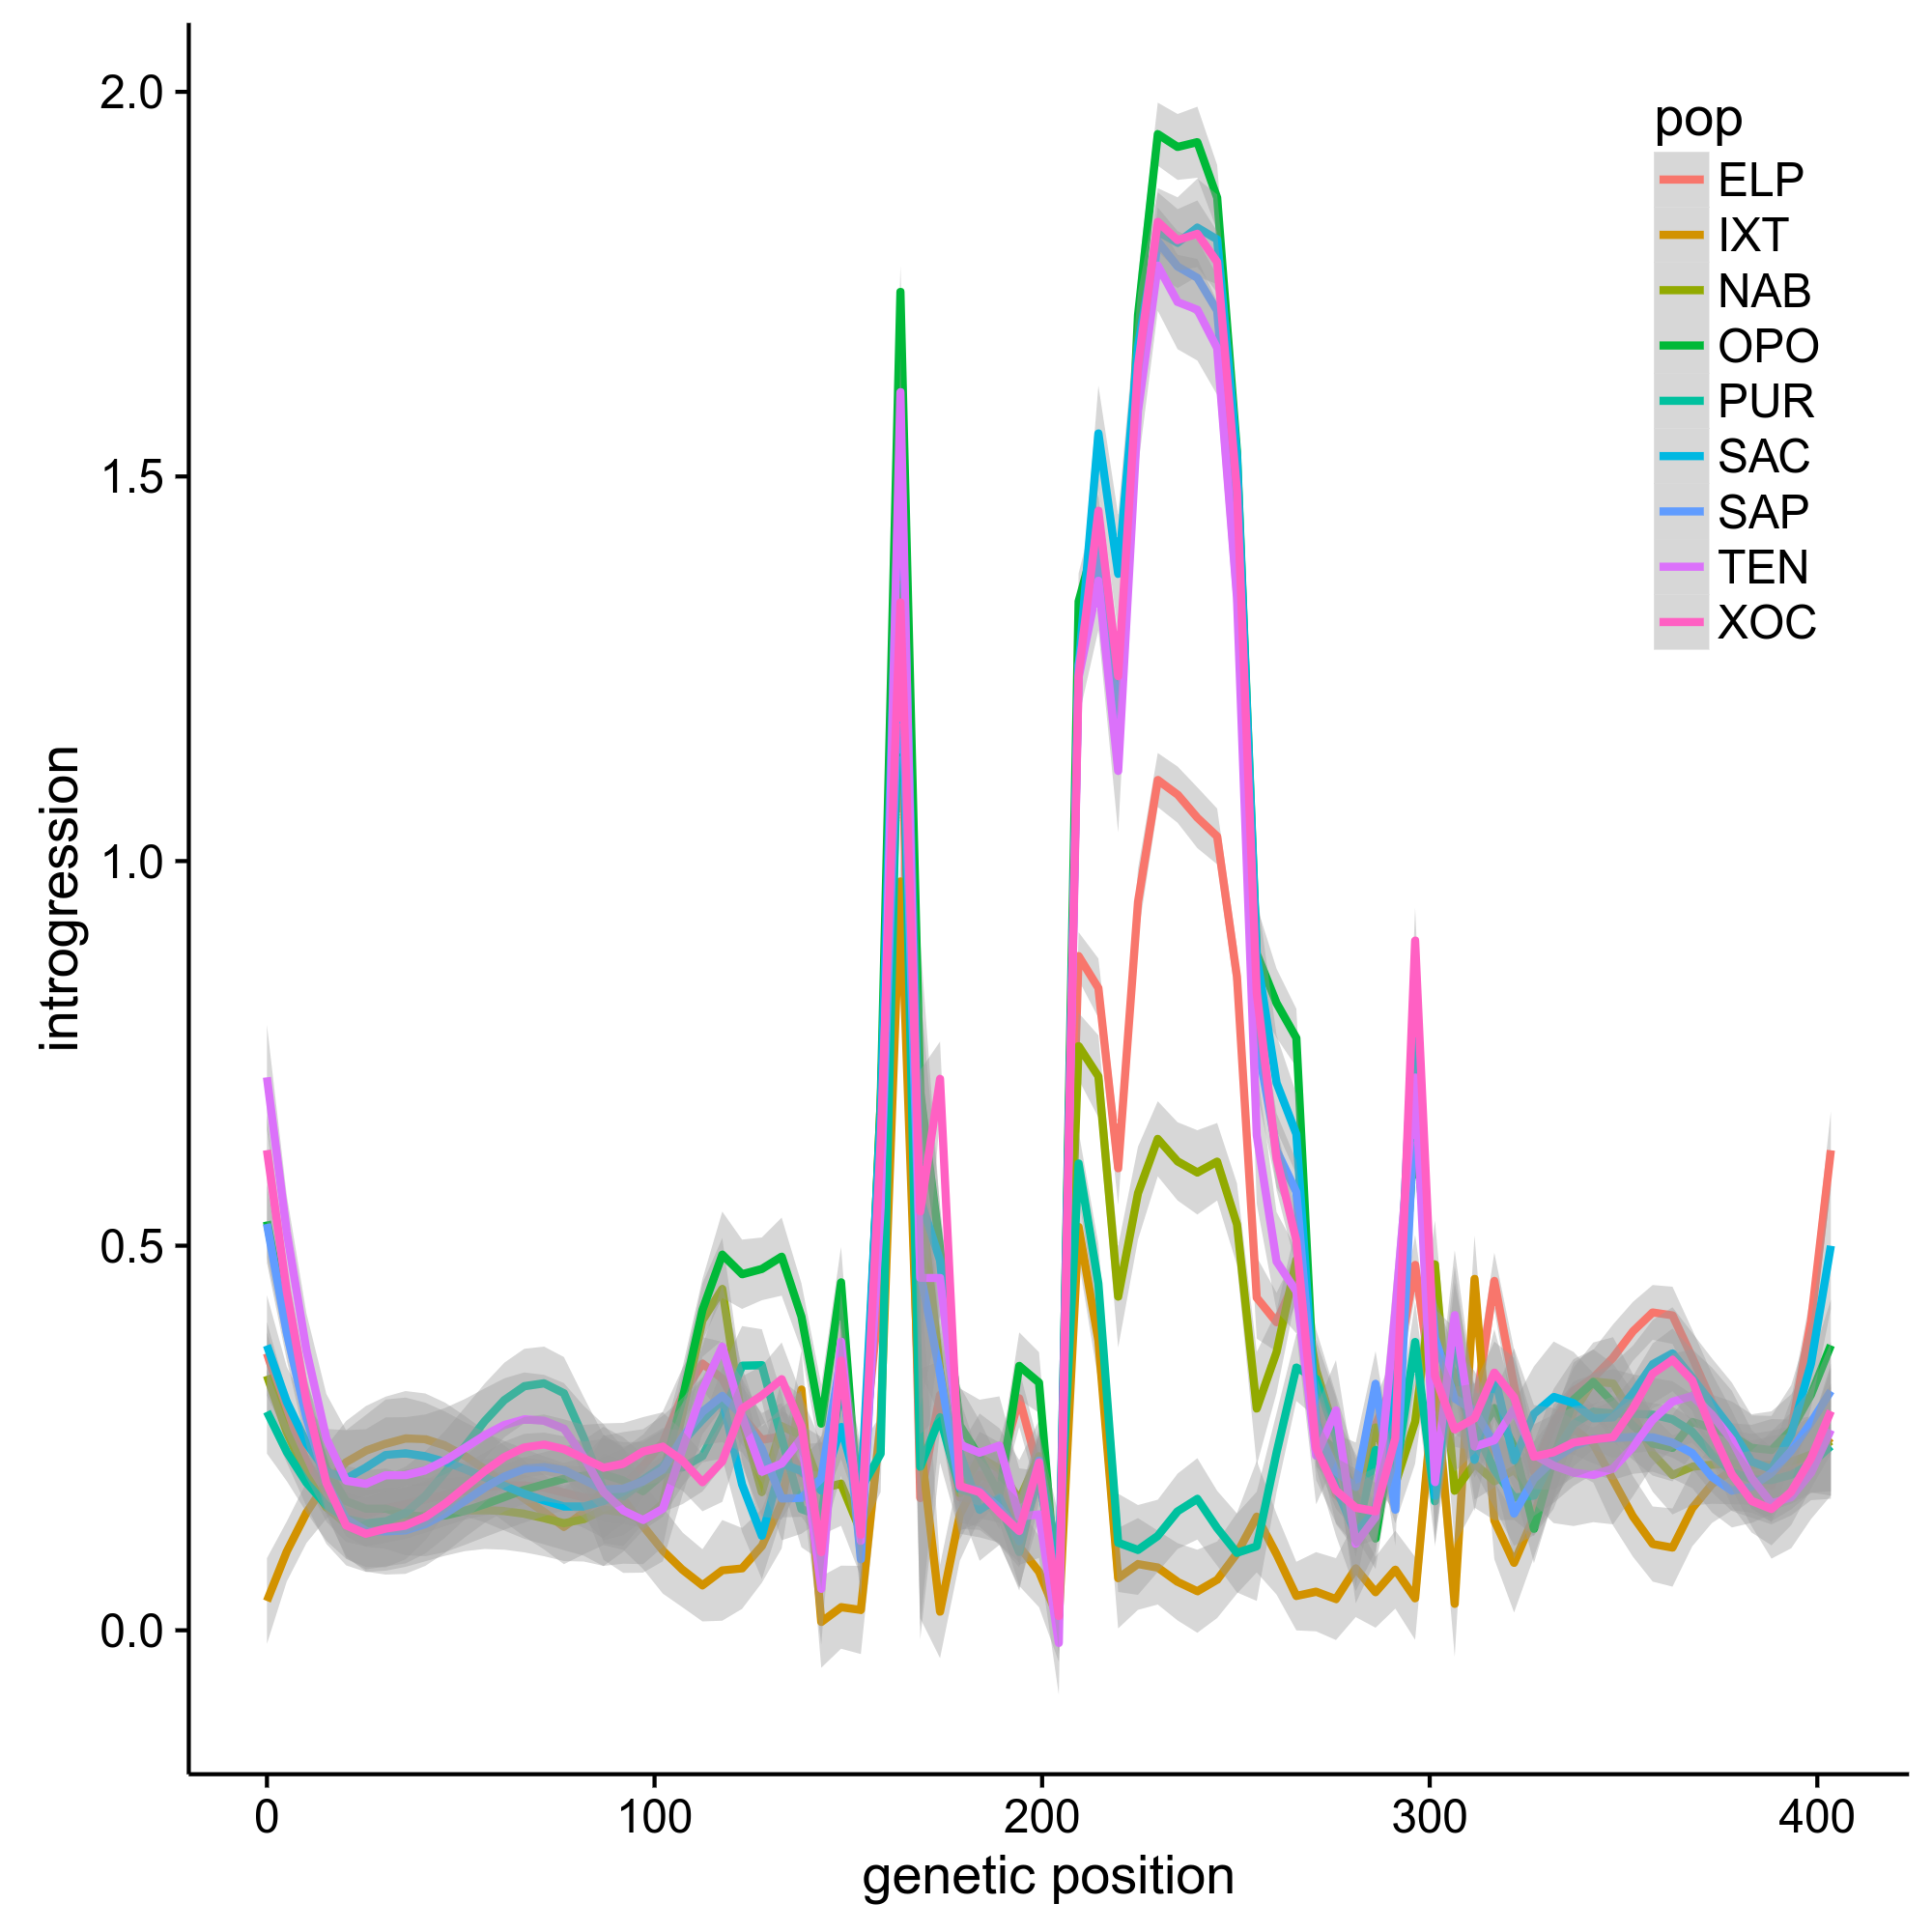
\includegraphics[width=17.35cm]{li_figure.png}
	\caption{Li's caption here.}
	\label{fig:introgressionMaize}
\end{figure}



\item{Barley:}
		
%Domesticated and wild barley belong to the same species, \emph{Hordeum vulgare}, and are capable of producing viable offpspring via hybridization \cite{von1995ecographical}.
Barley (\emph{Hordeum vulgare} subsp. \emph{vulgare}) was domesticated at least twice roughly 10,000 BP: once from the wild subsp. \emph{spontaneum} in the Fertile Crescent and once from subsp. \emph{spontaneum} var. \emph{agriocrithon} in Tibet \cite{takahashi1955origin, badr2000origin, oka2012origin, azhaguvel2007phylogenetic, haberer2015barley}.
\gmj{the source morrell2007genetic will be used to update this paragraph once we've worked out for sure that the second domestication of barley was in the Zargos mountains, rather than Tibet.  Also, this paper puts the earliest archaeological samples of barley at closer to 8500 calibrated years ago.}
%However, details of barley domestication are still somewhat unclear.
%Variety \emph{agriocrithon} is genetically diverse, and is found throughout much of the range of barley.
%Some have suggested that \emph{agriocrithon} may be the progenitor of six-rowed barley, the product of a hybridization between eastern and western cultivated barley, or a wild-domesticate hybrid \cite{staudt1961origin, zohary1959hordeum, murphy1982origin}\, but \cite{azhaguvel2007phylogenetic}\ dispute these theories, suggesting instead that it arose from ssp. \emph{spontaneum}, perhaps more than once (in Israel as well as in Tibet).
Presently, the distribution of subsp \emph{spontaneum} stretches from the eastern Mediterranean through the Middle-East to west-central Asia spanning clines in temperature, precipitation, soil type, and altitude \cite{nevo2010drought}.
%While little genetic investigation into spontaneous barley/\emph{spontaneum} hybrids \cite{ellstrand2003dangerous}.
Barley/\emph{spontaneum} hybrids are known to be fertile and are found spontaneously when wild and domesticated barleys co-occur.
In some cases, wild-to-crop introgression has been shown to occur over distances of more than a kilometer \cite{hillman2001new}.


%The barley domestication process has reduced the number of alleles in the domesticate to only 40\% of that found in wild barley, though there remains a great deal of phenotypic diversity among the wild barleys \cite{ellis2000wild}.
\mbh{I think here a more focused discussion of potential for adaptive introgression based on the Poets paper is needed}
The authors of \cite{Poets2015} used STRUCTURE to look for patterns of introgression from wild relatives in a dataset of 803 landraces, and found a high amount variability in the amount of contribution from wild relatives, as well as its location in the genome, within barley populations.
This is indicative of contribution from numerous wild populations.
Furthermore, the authors found that wild introgression contribution is generally greatest from geographically-proximate populations, and that introgressed regions might be combined from geographically-separate wild populations.
Low linkage disequilibrium and small blocks of identity by state indicate that these introgressed regions are old, perhaps dating back to the beginning of barley domestication.
As landraces and nearby wild relatives share similar genomic sequences, the introgressed regions that are exclusive to that landrace are more likely to contain adaptive alleles. 
Such alleles were not identified specifically, though wild-domesticate breeding experiments have shown that wild barleys have alleles for several important agronomic phenotypes, including powdery mildew resistance, brittleness, flowering time, plant height, lodging, and yield \cite{dreiseitl2017heterogeneity,von2006ab,handley1994chromosome}.

\item{Sunflower: }

The common sunflower (\emph{Helianthus annuus}) shows evidence of domestication in the eastern United States \cite{harter2004origin, wills2006chloroplast}\, with potential for a second domestication center in Mexico \cite{lentz2008sunflower}.
The pre-Columbian \emph{H. annuus} distribution of cultivated sunflower spanned much of the Great Plains, from what is now north-central Texas to Montana and North Dakota (see figure 1 of \cite{whitney2010adaptive}).
Domesticated sunflower has long lived in sympatry with wild relatives such as \emph{H. petiolaris} and \emph{H. bolanderi} and forms stable hybrid populations with these taxa \cite{schwarzbach2002likely, rieseberg1988molecular, welch2002patterns}.
Wild sunflowers are known to be locally-adapted, and weedy hybrid populations often share these adaptations \cite{kane2008genetics}.
However, the most striking example of adaptive introgression within \emph{Helianthus} is that of the cucumberleaf sunflower, \emph{H. debilis} ssp. \emph{cucumerifolius}.
\mbh{I believe \emph{H. annuus} ssp. \emph{texanus} is a wild sunflower, right?  If so, this is more an example of hybrid speciation rather then adaptive wild-to-crop gene flow}
Cucumberleaf sunflower is endemic to south-central Texas, and exhibits several adaptations to the region.
Introgressive hybridization imparted locally-adapted alleles from \emph{H. debilis} to \emph{H. annuus} via introgressive hybridization \cite{heiser1951hybridization}. 
These introgressed hybrids formed a new lineage of sunflower (\emph{H. annuus} ssp. \emph{texanus}, \emph{H. a. texanus} hereafter) which displays \emph{H. debilis}-like traits adaptive to south-central Texas climate and ecology.
These adaptive \emph{debilis}-like traits include resistance to herbivorous pests and an increased branching plant architecture, as well as higher overall fitness than \emph{H. annuus} (as measured by higher seed production \cite{whitney2006adaptive}).
Although H. annuus and \emph{H. a. texanus} are interfertile, \emph{H. a. texanus} displays persistent phenotypic differences from \emph{H. annuus} \cite{rieseberg2007hybridization}.


The genome of the common sunflower has been greatly influenced by introgression from wild relatives, due to both natural outcrossing events and concerted breeding efforts in crop improvement.
\emph{Helianthus} has several genes for downy mildew resistance, and each imparts resistance to one or more races of \emph{Plasmopara halstedii}, one of the most agronomically important diseases in sunflower cultivation \cite{cohen1973factors}.
Some of these downy mildew resistence genes were found in wild relatives (including \emph{H. argophyllus}, \emph{H. tuberosus}, and \emph{H. praecox}) and have been successfully bred into modern \emph{H. annuus} \cite{miller1991inheritance}.
PlArg, an allele found in wild silverleaf sunflowers (\emph{H. argophyllus}, inbred line Arg1575-2), confers resistance to all known (20 or more) races of downey mildew \cite{dussle2004pl}\, while others (Pl1-Pl11) are effective for one or more types \cite{rahim2002inheritance}.
Silverleaf sunflower has also been the focus of drought resistance breeding efforts \cite{saucă2010introgression}\ and \emph{Phomopsis} resistance breeding efforts \cite{besnard1997specifying}.
\emph{H. annuus} shows signs of persistent introgressive hybridization with \emph{H. petiolaris} with evidence of positive selection driving some of the genetic differentiation between the two species \cite{yatabe2007rampant}.


Recent investigations into the history of \emph{Helianthus} introgression have implemented genomic methods.
\cite{Baute2015} analyzed transcriptome sequence variation on cultivated and wild \emph{H. annuus}, \emph{H. petiolaris}, and \emph{H. argophyllus}.
Using STRUCTURE, these authors found that introgressions from wild relatives exist on every chromosome in at least one modern line, covering over 10\% of the genome.
Of particular note is the modern line RHA 274, a modern line which was bred with \emph{H. a. texanus} in the 1970s to restore a branching plant body architecture, which allows the plant to produce pollen for a longer period of time, increasing seed production.
RHA 274 has several large introgression from \emph{H. a. texanus}, including one at the site of HaGNAT, the domestication gene associated with branching.
These introgressed regions are not found in the non-branching lines Sunrise and VNIIMK8931, further suggesting that the \emph{H. a. texanus} introgressed regions are causative.











Notes for review:

http://biology.unm.edu/Whitney/Whitney%20Reprints/Whitney%20et%20al.%202006%20Am%20Nat.pdf

http://www.jstor.org/stable/pdf/2409227.pdf?refreqid=excelsior:a686b7f06f9daa2b89bd5a654dade3b4

file:///home/gjanzen/Downloads/Whitney_et_al-2010-New_Phytologist%20(2).pdf

http://onlinelibrary.wiley.com/doi/10.1111/j.1469-8137.2010.03234.x/epdf

https://biology.unm.edu/Whitney/Whitney%20Reprints/Scascitelli%20et%20al%202010.pdf

Genome scan of hybridizing sunflowers from Texas
(Helianthus annuus and H. debilis) reveals asymmetric
patterns of introgression and small islands of genomic
differentiation:

In contrast, coalescent analyses of long-term migration
rates imply that interspecific migration has been
more important than mutation in providing new genetic
variation in ssp. texanus populations. Immigration from
H. debilis cucumerifolius into ssp. texanus (M = 4.05;
Nem = 1.74) is higher than median estimates of intraspecific
migration rates in plants (Morjan and Rieseberg 2004) 
and only slightly lower than immigration from
ssp. annuus into ssp. texanus (M = 5.00). Immigration
rates from ssp. texanus into H. debilis cucumerifolius and
ssp. annuus are still higher (M = 6.30 and 7.29, respectively),
implying that the putative hybrid lineage serves
as a bridge for migration between the parental species.

One puzzle is
that the estimated immigration rate between the allopatric
taxa (H. debilis cucumerifolius and ssp. annuus) is
approximately comparable with that between the sympatric
taxa (H. debilis cucumerifolius and ssp. texanus ssp.
texanus). This observation may point to the effectiveness
of ssp. texanus as a bridge for the transfer of alleles
between H. debilis and ssp. annuus. An alternative explanation
is that the BAYESASS estimates are unreliable
because homoplasy of microsatellite alleles is high in
taxa with large-effective population sizes (Estoup et al.
2002) such as the annual sunflowers studied here.

Despite the apparent discrepancy between the results
from STRUCTURE and BAYEASS, several conclusions
can be made. Analyses with STRUCTURE support the
distinctness of ssp. texanus, as well as its clear inclusion
within H. annuus, as initially postulated by Heiser (1951).
Likewise, the STRUCTURE, MIGRATE-N and BAYESASS
analyses all confirm previous report of introgression
between H. annuus and H. debilis (Rieseberg et al.
1990, 2007) and suggest that the introgression is genomewide
when it occurs. Contrary to the Heiser’s scenario of
a recent Holocene origin of ssp. texanus, however, our
results are more consistent with a much longer history of
contact between H. annuus and H. debilis. Otherwise, it is
difficult to account for the presence of significant longterm
migration between currently allopatric populations
of ssp. annuus and H. debilis cucumerifolius. This revised
scenario makes sense in the light of numerous glacialinterglacial
cycles over the past million years (Hewitt
2000), which probably resulted in intermittent contact
between H. annuus and H. debilis, with the last contact
likely occurring during the Wisconsin glaciation,
18 000 BP. The current contact between the species differs
from the previous ones in that it appears to have been
human-aided. Possibly, some of the molecular evidence
of introgression, particularly into allopatric populations,
stems from past periods of contact.

One of the four outlier loci, HT0414, is associated
with a heat-shock protein and was previously shown to
have been the target of selection in H. annuus ssp. annuus
salt marsh populations from the state of Utah
(Kane and Rieseberg 2007), as well as in weedy sunflower populations
from several different locations across the USA
(Kane and Rieseberg 2008). In this study, populations of
ssp. annuus from Kansas, Nebraska and Oklahoma
monomorphic for a single allele, whereas populations
of H. debilis and other populations of ssp. annuus are
considerably more polymorphic. These results imply
that HT0414 may be involved in adaptation to a range
of different habitats or to conditions shared by several
different habitats (Kane and Rieseberg 2008).








%The species \emph{H. annuus} is a versatile species, capable of adapting to a wide range of environments across the Americas, Europe, Asia, and Australia \cite{kane2008genetics}.
%This versatility may be due in part either to phenotypic plasticity or genetic adaptability \cite{maron2004rapid}.





%whitney2006adaptive
%"these results suggest that introgression of biotic resistance traits was important in the adaptation of H. annuus to central and southern Texas."
%fitness (seed production) high in texanus than in annuus
%identified two pests to which resistance was imparted and important
%Discussion points: 1. texanus has higher fitness than annuus in central texas.
%2. texanus shared traits more in common with debilis than with annuus (herbivore resistance)
%3. 2 of the three traits from point two above are important for adaptation to life in central south Texas.
%The authors ask why these pest-resistance genes have not spread further north beyond this range.  They are uncertain, but conjecture that negative pleiotrophic effects are at play.

%whitney2010adaptive
%"We demonstrate that introgression has altered multiple aspects of the H. annuus phenotype in an adaptive manner, has affected traits relevant to both biotic and abiotic environments, and may have aided expansion of the H. annuus range into central Texas, USA."
%This paper really does show that this case of natural introgression was adaptive.
%The companion paper (2006 Whitney) will likely show the same thing, but I haven't read it yet.

%scascitelli2010genome
%"long-term migration rates were high, genome-wide and asymmetric, with higher migration rates from H. annuus texanus into the two parental taxa than vice versa."
%"H. annuus texanus may serve as a bridge for the transfer of alleles between its parental taxa."
%"contradict recent theory suggesting that introgression should predominantly be in the direction of the colonizing species."

%rieseberg2007hybridization
%this is a very good review.  i think i should use it for the table.
%they also show that traits were imparted from debilis to texanus, and that these are adaptive.  i think they also show genetic evidence, but i'm not sure.






\item{Asian Rice:}

The story of Asian rice (\emph{Oryza sativa}) domestication is still debated.
A recent investigation pointed to a single domestication occurring 8,200-13,500 BP in the Yangtze Basin in China from the wild species \emph{Oryza rufipogon} (\emph{rufipogon} hereafter), with later divergence of the two prominent varietal groups, \emph{japonica} and \emph{indica} \cite{molina2011molecular}.
\cite{vaughan2008evolving} support this view, noting that present-day patterns of rice variation could be explained by a single domestication event in a population with high standing variation, followed by dispersal into sympatry with locally-adapted wild relatives in diverse environments, genetic admixture, and selection for adaptive alleles.
On the other hand, both genetic and archaeobotanical evidence point toward independent domestications of \emph{japonica} and \emph{indica} in the Yangtze Basin and the Indian Ganges plain, respectively \cite{fuller2010consilience}.
An alternative explanation, as described by \cite{Huang2012}, suggests an initial domestication of \emph{japonica} in China followed by formation of the \emph{indica} group through hybridization of \emph{japonica} and local \emph{rufipogon} populations in Southern and South-eastern Asia.
Adaptive introgression may in fact be the signal interpreted as independent domestications.



The high genetic diversity within domesticated rice is likely due to introgression from wild relatives both within the domestication center(s) and in new environments where rice has dispersed \cite{second1982origin}, and gene flow between domesticated Asian rice and its wild relatives outside of the Yangtze Basin could have imparted locally adaptive traits \cite{vaughan2008evolving}.
The wild relatives \emph{rufipogon} and \emph{nivara} both maintain high phenotypic diversity and exhibit locally-adaptive traits.
\emph{Rufipogon} reproduction can be either primarily sexual or vegetative, and whereas \emph{rufipogon} is adapted to forested wetland environments, \emph{nivara} is adapted to dryer conditions and has life cycle adaptations to survive grazing pressure.
Likewise, domesticated rice varieties display patterns of local adaptation.
For examples, two of the domesticated rice deepwater varieties (\emph{rayada} and \emph{ashwina}) are said to be selected for the environment along the Ganges river, the \emph{japonicas} are split into temperate and tropical subgroups, and the \emph{indicas} are best suited for lowland environments.
Gene flow between these wild and cultivated rices, though asymmetrical, is exceedingly common, producing nuisance weedy hybrids when the two are grown in sympatry.



To date, research into adaptive introgression in the domestication of rice has been insufficient to detect clearly-supported examples.
\cite{zhao2010genomic} used a SNP panel and STRUCTURE analysis to uncover patterns of population structure, admixture, and introgrogression within domesticated rices, and the authors emphasize the importance of similar research that includes wild rice accessions.
There are perhaps some practical reasons why research has not yet been devoted to this inquiry.
As with many other domesticated crops, gene flow between wild and domesticated rices is highly asymmetric (estimates of wild rice admixture in domesticated rice are less than 5 percent \cite{wang2017asian}).
This asymmetry is due in part to the closed floret architecture of the domesticated rice, which hinders outcrossing.
However, during early domestication, introgression may have been more prevalent than at present because barriers to crop-to-wild introgression may have been less severe and because the inbreeding reproductive system of rice would not have been as firmly established \cite{vaughan2008evolving}.
Furthermore, the contemporary distribution of wild rice does not capture the range and diversity of wild rice during early domestication and range expansion of rice.

%Introgression into indica is expected to be more likely than japonica, due to the higher degree of sympatry between indica and its wild relatives.

%note from Asian wild rice is a hybrid swarm with extensive gene flow and feralization from domesticated rice:
%Cite this paper to talk about how the ranges of the several subspecies of domesticated rice are distinct/sometimes overlap.  The paper makes the point that this overlap helps facilitate gene flow.









\end{enumerate}

	

	
	
	
	
	
	
	
	



\begin{table}
\rowcolors{2}{white}{gray!25}
\begin{center}
\caption{List and brief description of recently developed methods and examples of empirical studies employing these methods.} \label{tab:tools}
\begin{tabular}{llll}
\\\toprule  
\rowcolor{white}
{\bf methods}	& {\bf data type } &	{\bf reference} &  {\bf empirical studies } \\ \midrule

\rowcolor{gray!25}
{\emph{\bf chromosome paiting}} &   &   &   \\
\rowcolor{gray!25}
Hapmix	& phased haplotype; reference panel		& Price et al. 2009	&  Hufford et al. 2013;  Suarez et al. 2016 \\ 
\rowcolor{gray!25}
RASPberry &	phased haplotype &	Wegmann et al. 2011	 & Christe et al. 2016 \\
\rowcolor{gray!25}
MultiMix & phased/unphased genotype; reference panel &	Churchhouse and Marchini 2013 &	Eyheramendy et al. 2015 \\
\rowcolor{gray!25}
PCAdmix	 & phased haplotype	 & Brisbin et al. 2012	 & Moreno et al. 2014; Pugach et al. 2016 \\
\rowcolor{gray!25}
LAMP  &	phased haplotypes; reference panel	 & Sankararaman et al. 2008	 & Patterson et al. 2012 \\

\rowcolor{white}
{\emph{\bf phylogenetic relationship}} &   &   &   \\
\rowcolor{white}
ABBA-BABA/D-statistics	 & biallelic SNP  &	Durand et al. 2011	 &  Heliconius Genome Consortium 2012 \\
\rowcolor{white}
fd statistic &	biallelic SNP &	Martin et al. 2015  &	Malinsky et al. 2015; Zhang et al. 2016 \\ 
\rowcolor{white}
five taxon D statistics	& biallelic SNP	&  Pease and Hahn 2015	& Fontaine et al. 2015; Pease et al. 2016 \\

\rowcolor{gray!25}
{\emph{\bf divergence}} &   &   &   \\
\rowcolor{gray!25}
Gmin &	biallelic SNP	&  Geneva et al. 2015	&  Kingan et al. 2015 \\
\rowcolor{gray!25}
RNDmin	& phased haplotype	& Rosenzweig et al. 2016	&  NA \\
\rowcolor{gray!25}
(see .tex file for comment) & biallelic SNP & Racimo et al. 2016 & Sams et al. 2016 \\

%I was not able to add Li's entry to this cell without errors.  I'll put her entry in the line below:
%U_{A,B,C(w,x,y)} and Q95_{A,B,C(w,y)}

\rowcolor{white}
{\emph{\bf population structure related}} &   &   &   \\
\rowcolor{white}
fineStructure &	phased haplotype &	Lawson et al. 2012	& Skoglund et al. 2015 \\
\rowcolor{white}
Globetrotter &	phased haplotype &	Hellenthal et al. 2014 & Scott et al. 2016 \\
\end{tabular}
\end{center}
\end{table} 





\begin{table}
\centering
\begin{adjustbox}{width=1\textwidth}
\small
\label{my-label}
\begin{tabular}{|p{5cm}|p{5cm}|p{2.6cm}|p{2.6cm}|p{2.6cm}|l|}
\hline
Crop & Compatible Wild Relatives & Hybrids and/or Hybridization & Evidence of Crop Introgression & Evidence of Adaptiveness & Source \\ \hline \hline
Maize (\emph{Zea mays} subsp. \emph{mays}) & \emph{Z. m.} subsp. \emph{mexicana}, \emph{Z. m. } subsp. \emph{parviglumis} & X & X & X & \cite{hufford2013genomic} \\ 
\hline 
Asian Rice (\emph{Oryza sativa}) & \emph{O. rufipogon} & X & X & X & \cite{Huang2012} \\ 
\hline
Barley (\emph{Hordeum vulgare}) & \emph{H. v.} subsp. \emph{spontaneum} & X & X & X & \cite{Poets2015} \\ \hline
Sunflower (\emph{Helianthus annuus}) & \emph{H. argophyllus}, \emph{H. bolanderi}, \emph{H. debilis}, \emph{H. petiolaris} & X & X & X & \cite{rieseberg2007hybridization}\\ 
\hline
Cassava (\emph{Manihot esculenta}) & \emph{M. glaziovii} & X & X & X & \cite{bredeson2016sequencing} \\ 
\hline
Potato (\emph{Solanum tuberosum}) & many & X & X & X & \cite{johns1986ongoing, gavrilenko2013genetic} \\
\hline
Tomato (\emph{Solanum lycopersicum}) & \emph{S. pimpinellifolium} & X & X & X & \cite{rick1958role} \\
\hline
Olive (\emph{Olea europaea} ssp. \emph{europaea} var. \emph{sativa}) & \emph{O. e.} ssp. \emph{europaea} var. \emph{sylvestris} & X & X & & \cite{diez2015olive} \\ 
\hline
Soybeans (\emph{Glycine max}) & \emph{G. soja} & X & X &  & \cite{lam2010resequencing} \\ 
\hline
Common Bean (\emph{Phaseolus vulgaris}) & \emph{P. v.} var. \emph{aborigineus, P. v.} var. \emph{mexicanus} [[not in this source]]& X & X &  & \cite{papa2003asymmetry} \\
\hline
Grapes (\emph{Vitis vinifera} subsp. \emph{vinifera}) & \emph{V. v.} subsp. \emph{sylvestris} & X & X &  &  \cite{myles2011genetic} \\
\hline
Sorghum (\emph{Sorghum bicolor} subsp. \emph{bicolor}) & \emph{S. b.} subsp. \emph{arundinaceum, S. b.} subsp. {drummondii} & X & X &  & \cite{aldrich1992patterns} \\
\hline
Wheat (\emph{Tritium monococcum, T. dicoccum, T. aestivum}) & \emph{T. m. boeoticum, T. dioccoides, T. urartu, Aegilops speltoides, A. tauschii} & X & X &  & \cite{zohary1969wild} \\
\hline
Apple (\emph{Malus domesticus}) & \emph{M. sylvestris}, \emph{M. orientalis}, \emph{M. baccata}, \emph{M. sieversii}  & X & X & & \cite{cornille2012new} \\
\hline
\end{tabular}
\end{adjustbox}
\end{table}

\begin{figure}[h]
	\centering
	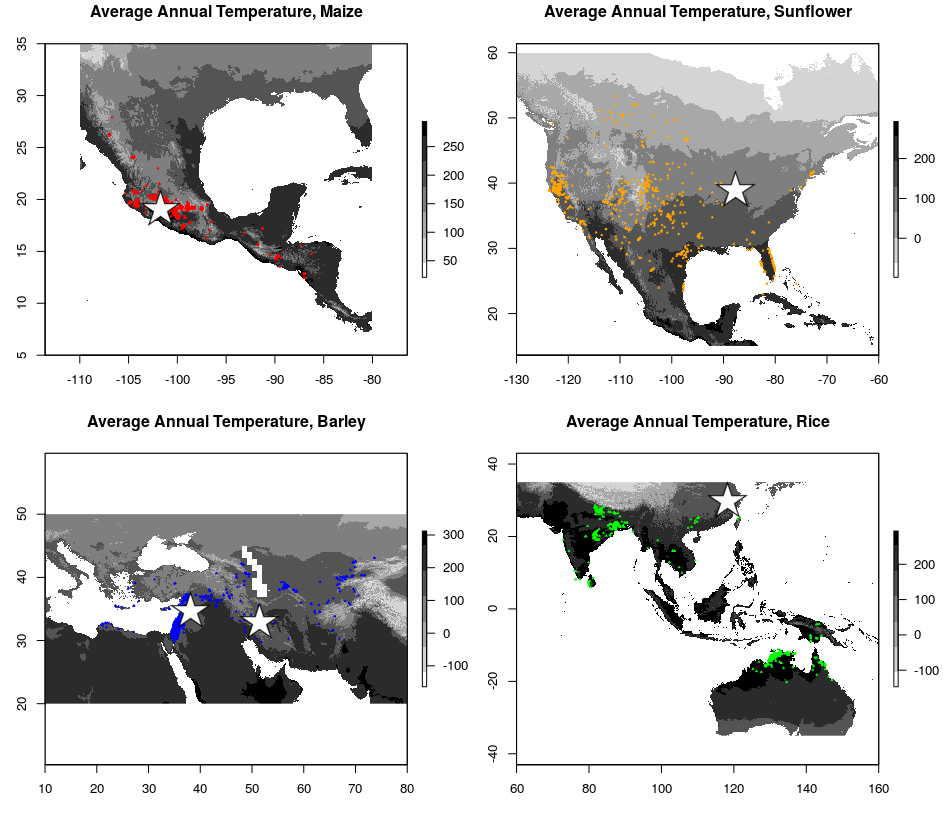
\includegraphics[width=17.35cm]{par_figure_stars.png}
	\caption{Map of the natural ranges of wild relatives of four domesticated crops, overlayed with average annual temperature.}
	\label{boxplot:map}
\end{figure}

\begin{figure}[h]
	\centering
	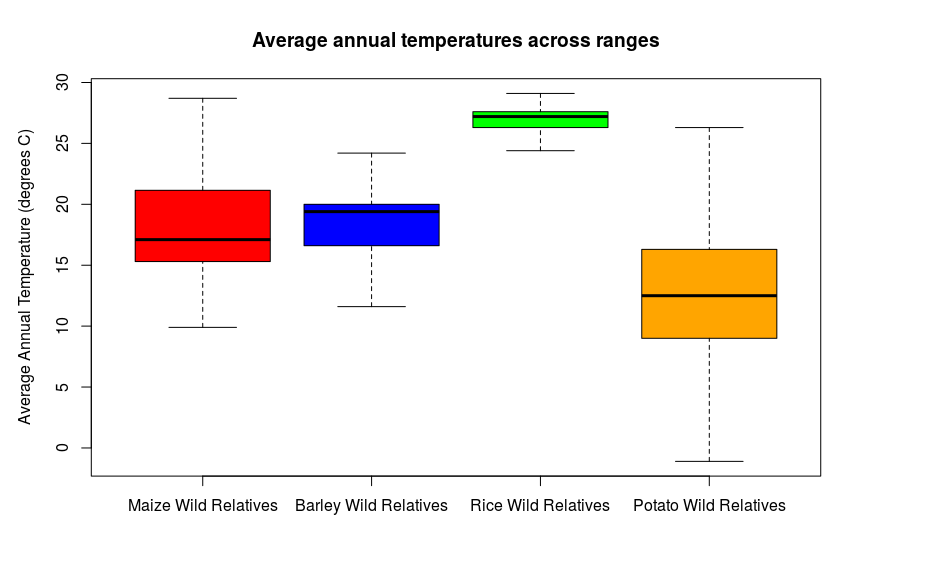
\includegraphics[width=17.35cm]{boxplot.png}
	\caption{The distribution of average annual temperature experienced in the geographic home ranges of wild relatives interfertile with four crops}
	\label{fig:map}
\end{figure}

\section*{Re-evaluating concepts of domestication}

A framework in which crops are domesticated from a single wild population or even a single species is an oversimplification when introgression during the geographic expansion of crops is extensive.
The addition of ongoing gene flow to our understanding of crop demography could bear importantly on fundamental questions of crop domestication:

\subsection*{What is the progenitor of a crop?}
Depending on the extent of post-domestication gene flow with new wild relatives, identification of a crop's progenitor can be complicated or completely confounded.
The level of divergence of a crop from newly encountered populations and species will decrease due to introgression, a signal that could be mistaken for origin rather than gene flow.
For example, when determining a single origin of maize from \emph{parviglumis}, Matsuoka and colleagues \cite{matsuoka2002single} identified a paradox: while \emph{parviglumis} is found exclusively in the lowlands of southwest Mexico, maize with allele frequencies most similar to \emph{parviglumis} was found in the highlands of the Mexican Central Plateau.
Several years later, van Heerwaarden \emph{et al.} \cite{vanHeerwaarden2011} resolved the paradox by determining widespread introgression in the highlands from \emph{mexicana}, which is closely related to \emph{parviglumis}, has caused maize from this region to appear ancestral.
Similarly, extensive post-domestication adaptive introgression from  potato wild relatives long obscured this crop's origin.
Recent work has shown that, following the original domestication event in the central Andes from \emph{Solanum tuberosum}, potato received introgression from as many as four additional species during colonization of the highest elevations of the Andes and the lowlands of the Chilean coast \cite{Spooner2014, Gavrilenko2013}.
Beyond confounding detection of progenitor taxa, extensive introgression may necessitate a reevaluation of crop origins.
In cases like maize and potato it is important to recognize the substantial contributions of introgressing taxa to the genetic base of modern crops.
Broad recognition of the role these wild relatives have played in crop adaptation could further their use in breeding and elevate their conservation status.

\subsection*{When was a crop domesticated?}
Estimates of the timing of domestication based on levels of sequence divergence may be affected when introgressed haplotypes are included.
The directionality of this effect is likewise dependent on $N_e$ of the donor population.

\subsection*{How was genome-wide diversity impacted by a domestication bottleneck?}
Estimates of the initial domestication bottleneck may be skewed when introgression is not considered.
Chromosomal regions experiencing introgression may have an altered effective population size ($N_e$) relative to non-introgressed regions depending on diversity within the donor taxon.
For example, introgression from wild taxa with historically high $N_e$ will lead to underestimates of the strength of the domestication bottleneck.
Conversely, if the donor population has a relatively small effective population size, the opposite bias may be imposed upon bottleneck estimations.
In most cases, the effective population size of the domesticated crop will be lower than that of the wild progenitor and wild relative populations.

\subsection*{What candidate genes were targeted by selection during domestication?}
Loci under selection during domestication are often identified based on signatures of substantially-reduced nucleotide diversity in the domesticated taxon relative to the wild progenitor and high allele frequency differentiation between these taxa.
Introgression may alter these signatures and confound detection of domestication loci.

%\lwang{I donot quite understand this point. So, it is assumed that the introgressed haplotype has higher diversity, which renders difficulty to detect selection in such regions, right? But the case in maize is that even the introgressed haplotypes had higher diversity, but as selection has act long time on the region, the observed current diversity has already been reduced.}

%\gmj{It may not fit here perfectly, but we might consider a point about how crop-wild introgressions can also mask or obscure even the true progenitor species and center(s) of domestication.  The examples of potato and tomato domestication comes to mind; in potato, persistent and thorough interbreeding with a complex of wild relatives during domestication probably make it impossible to identify a single progenitor (if ever there was one), and in tomato, widescale recent introgression between two or three wild relatives confound attempts to identify which is the progenitor, and therefore the center of domestication as well.}










\section*{Future studies in crop-wild introgression}

Research has so far shown that adaptive crop-wild introgression has played a significant role in the domestication histories of many agronomically-important crops.
However, the dynamics of the process in these cases are not yet fully understood.
To what extent does the level of introgression across taxa depend on divergence time and/or mutation load between donor and recipient taxa?
Can colonizing species and/or hybrid swarms serve as bridges for gene flow between previously allopatric taxa?
At what geographic scale does adaptive introgression occur?
Is introgression frequently restricted to very local populations, or is it often seen over broad geographic ranges?
To what extent does this depend on the slope of environmental gradients such as temperature, precipitation, and elevation?
How did the conscious, subconscious, and unconscious decisions of early farmers facilitate or hinder adaptive introgression into their crops during early domestication?
How do the practices of contemporary farmers affect the process of adaptive introgression today?

Additional study of introgression in agroecosystems could lead to advances in both basic and applied genetics, and specifically the continued improvement of modern crops.
Loci underlying the domesticated phenotype can be more clearly identified by removing the confounding population genetic signal of introgression.
These loci are potentially beneficial targets for crop improvement.
Furthermore, adaptive introgression that is clearly tied to a specific environment may include beneficial alleles that can be utilized in crop breeding.








\section*{Conclusions}

The study of crop domestication has been revolutionized by the advent and application of genomic tools.
The genomes of crops and their wild relatives tell a story of give-and-take that extends well beyond the initial stages of domestication.
Likewise, population genetic theory reinforces the proclivity of wild relatives to provide advantageous, locally-adapted alleles to crops as they disperse beyond their domestication centers into new geographies with new ecological pressures and niches.











\bibliography{bib_gj}

\end{document}


\end{document}



